%\chapter{Desarrollo de propuesta de prototipo}\label{cap:capitulo4}

%---------------------------------------------------------------------------
\subsection{Creación de conjunto de datos de entrenamiento y adaptación de nanoGPT}\label{section:Creación de conjunto de datos con fuentes de internet} 
El conjunto de datos contiene recomendaciones y prácticas de seguridad clasificadas por categorías como amenazas, ataques y malware, figura \ref{figure:Conjunto de datos}. Esta clasificación permite que el modelo mejore clasifique mejor la entrada de texto dada.
\begin{figure}[H]
   \centering % figure is centered on the page
       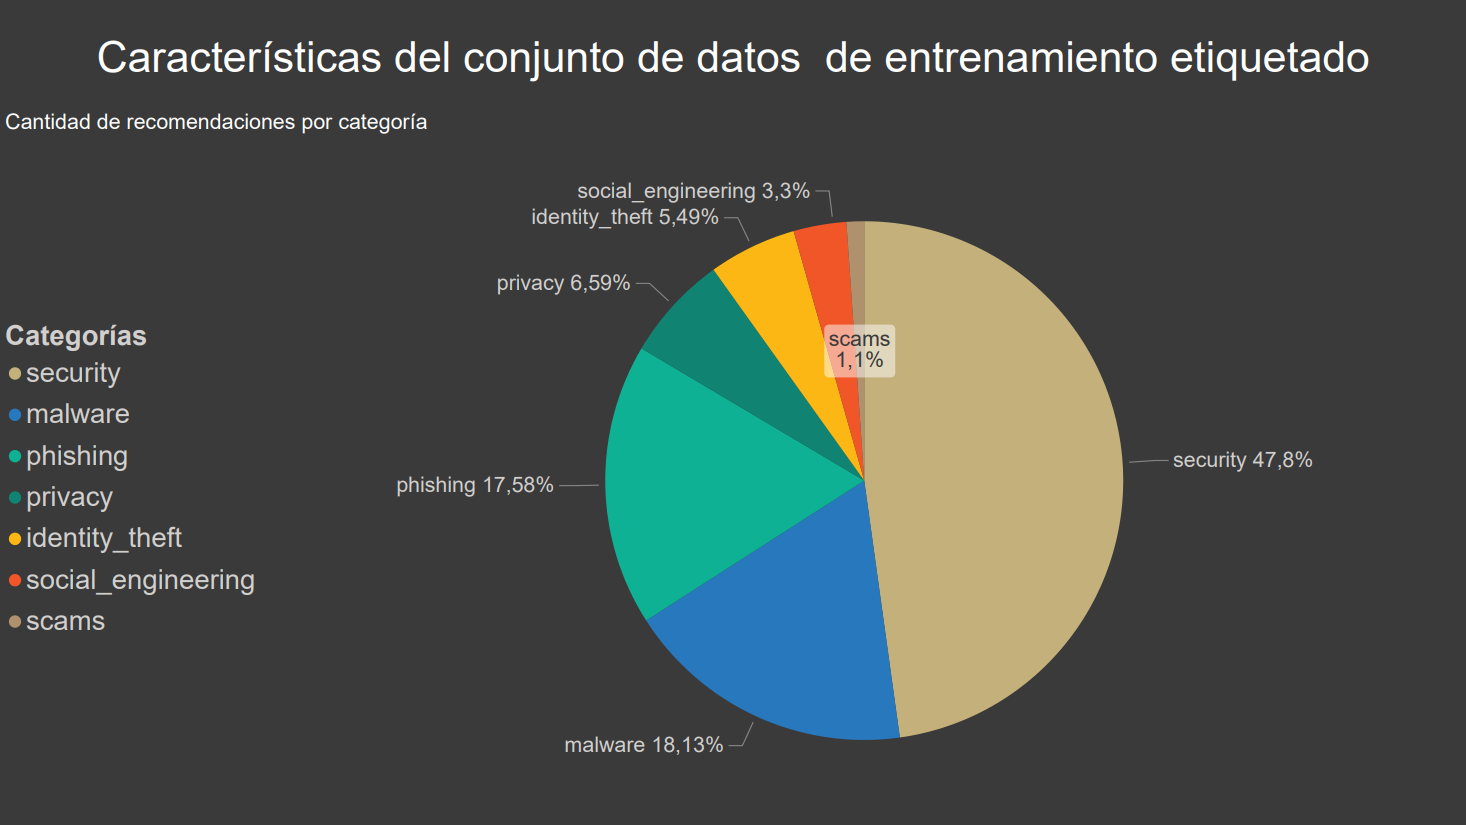
\includegraphics[width=0.6\linewidth]{./doc/Conjunto de datos etiquetado.png} 
   \caption{Características del conjunto de datos etiquetados \cite{}}
  \label{figure:Conjunto de datos}  % assign a unique label to each figure 
\end{figure}
%---Parrafo
Este se extrae desde el archivo CSV con el uso de la librería pandas a un dataframe. Figura \ref{figure:Extracción de datos del csv}.\cite{Reiss2021}
\begin{figure}[H]
   \centering % figure is centered on the page
       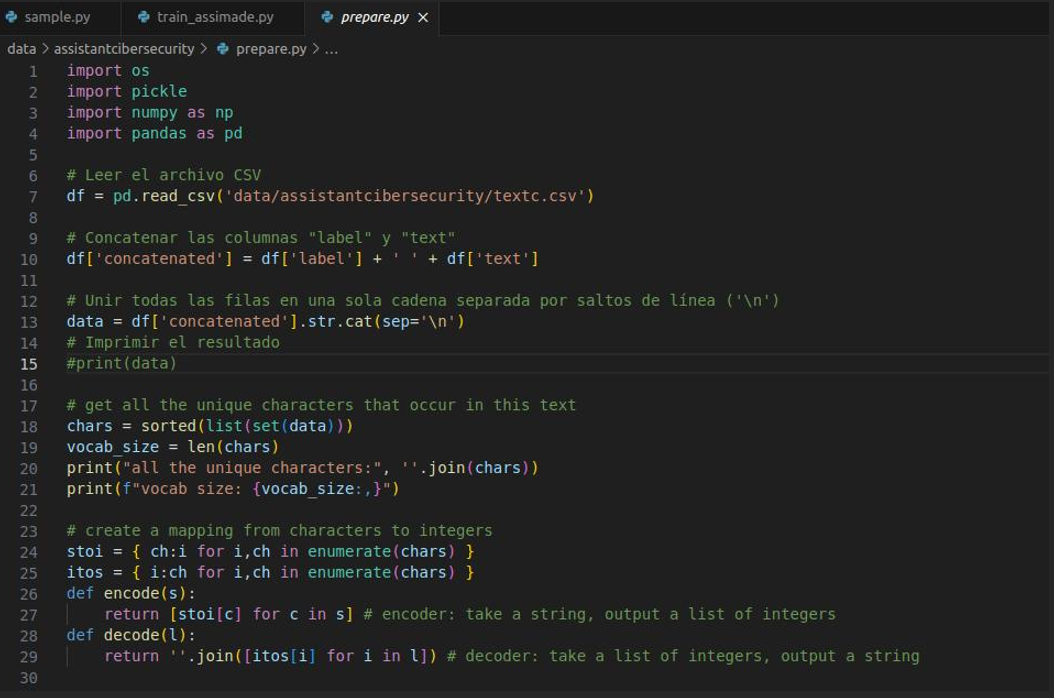
\includegraphics[width=0.6\linewidth]{./doc/02-cr.png} 
   \caption{Configuración para extraer el conjunto de datos en un dataframe y preparación de los datos.  \cite{}}
  \label{figure:Extracción de datos del csv}  % assign a unique label to each figure 
\end{figure}
\clearpage
Para el entrenamiento con NanoGPT se crean las carpetas del conjunto de datos, se realiza el proceso de mapeo de caracteres a enteros también llamado vectorización para representar los datos de texto en secuencias de números. \cite{GenerGediz2020}
En la figura \ref{figure:Etapa de encoder}
\begin{figure}[H]
   \centering % figure is centered on the page
       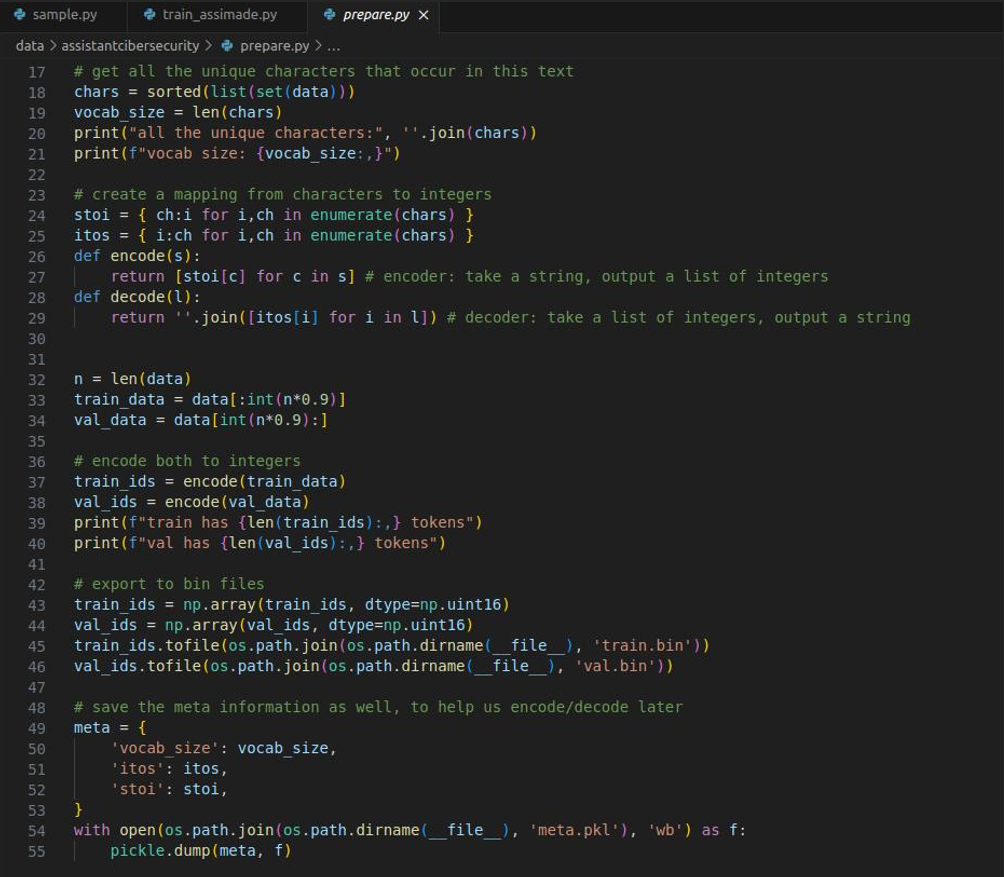
\includegraphics[width=0.6\linewidth]{./doc/03-cr.png} 
   \caption{procesamiento crea  ficheros de validación, entrenamiento y un meta modelo de apoyo.  \cite{}}
  \label{figure:Etapa de encoder}  % assign a unique label to each figure 
\end{figure}
%Parrafo-----
El procesamiento anterior crea ficheros de validación, entrenamiento y uno que contiene metadatos de los diccionarios para transformar de índices a palabras para apoyo al proceso de condificación y decodificación.
\begin{figure}[H]
   \centering % figure is centered on the page
       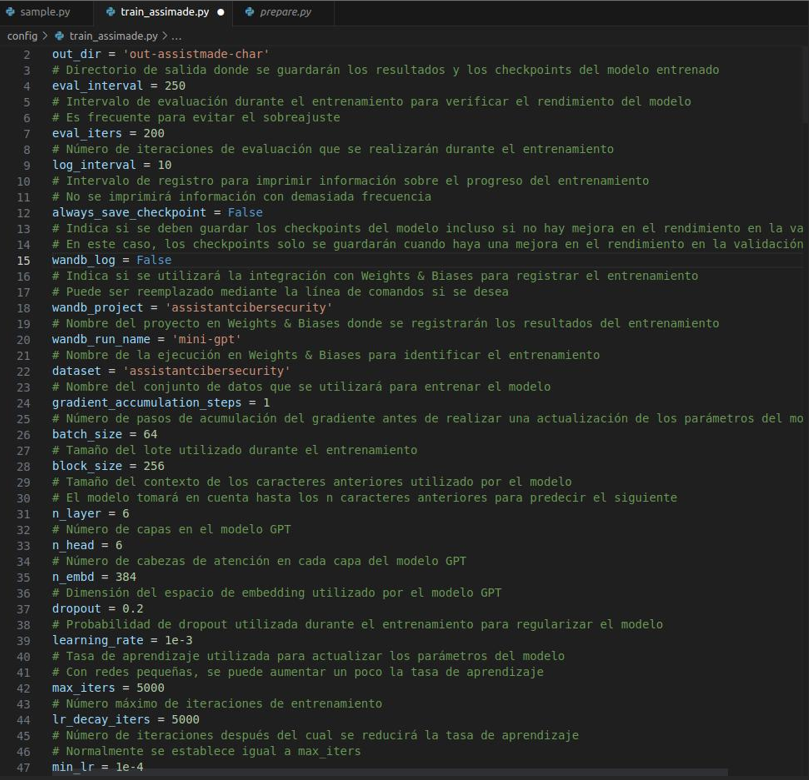
\includegraphics[width=0.6\linewidth]{./doc/04-cr.png} 
   \caption{Configuraciones y parámetros de entrenamiento que crea los directorios de salida para el modelo entrenado.  \cite{}}
  \label{figure:Configuraciónes de parámetros}  % assign a unique label to each figure 
\end{figure}
\clearpage
%---------------------------------------------------------------------------
\subsection{Configuración de los parámetros del código y entrenamiento}\label{section:Configuración y entrenamiento} 
Posteriormente se configuran dos modelos de prueba con variaciones de parámetros basados intervalos de entrenamiento, tamaños de bloque de texto procesado, cantidad de lotes en paralelo, ciclos de entrenamiento. 
Estas se realizado sobre la CPU, por lo que las configuraciones están centradas en entrenamientos de bajo rendimiento, el propósito es verificar configuraciones que permitan al modelo clasificar la entrada de texto y el conjunto entrenado.
\begin{enumerate}
	\item El tamaño de lote permite configurar cantidad de ejemplos que se procesan de forma paralela.
	\item Tamaño en bloques de permite configurar la dimensión del vector que representa al texto ingresado de forma secuencial.
	\item Configuración de las número de capas de la red y número de capas de atanción por cada capa de la red neuronal.
	\item Los vectores de incrustación para representar las palabras numéricamente vectores y generar resultados relacionados.
	\item Configuración de la red neuronal a 4 capas y 4 capas de atención que dan al modelo capacidad para asignar pesos del entrenamiento. 
	\item El tamaño de los vectores permiten crear una mayor representación de cantidades de palabras en la oración  para identificar representaciones significativas en un texto transformado.
	\item Por último el parámetro para establecer las iteraciones de entrenamiento se establecen en 3000. 
\end{enumerate} 
\begin{table}[H]
	\centering
	\begin{tabular}{|c|c|c|c|c|c|c|c|}
		\hline
		\textbf{Configuración} & \textbf{log\_interval} & \textbf{block\_size} & \textbf{batch\_size} & \textbf{n\_layer} & \textbf{n\_head} & \textbf{n\_embd} & \textbf{max\_iters} \\
		\hline
		Configuración 1 & 1 & 64 & 12 & 8 & 8 & 128 & 1000 \\
		Configuración 2 & 5 & 128 & 32 & 4 & 4 & 256 & 3000 \\
		\hline
	\end{tabular}
	\caption{Configuraciones de los modelos}
	\label{tab:configuraciones}
\end{table}

%-------------------------------------------------------------------------------
%------------------------------------------------------------------------------

\subsubsection{Configuración parámetros para entrenamiento}\label{section:Configuración de los parámetros del código} 
En esta sección se asignan a los parámetros mediante la ejecución del entrenamiento con en remplazo de las variables. Esto se realiza ejecutando el python y asignando los valores de las variables al ejecutar el archivo de entrenamiento.
\subsection{Configuración 1}\label{section:Configuración de los parámetros del código} 
\begin{itemize}
	\item   Objetivo: Con esta configuración se busca mayor cantidad de parámetros en el modelo reduciendo de bloque además se aumenta cantidad de capas de red y capas de atención.
\end{itemize}
\begin{figure}[H]
	\centering % figure is centered on the page
	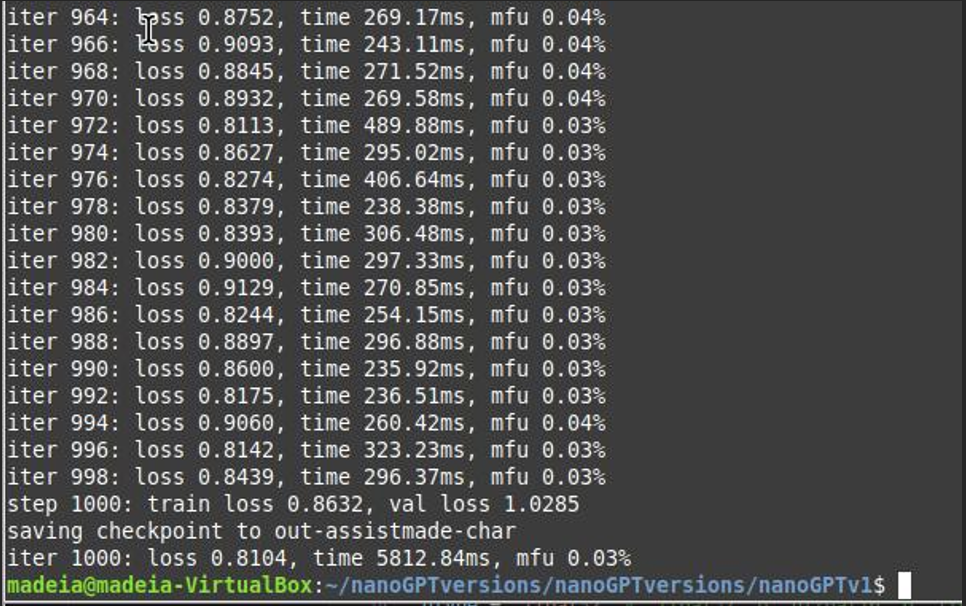
\includegraphics[width=0.60\linewidth]{./rp/15-cp.png} 
	\caption{Proceso de entrenamiento de modelo 1\cite{}}
	\label{figure:Resultado 1}  % assign a unique label to each figure 
\end{figure}
%------------------------------------------------------------------------------
\subsection{Configuración 2}\label{section:Configuración de los parámetros del código} 
\begin{itemize}
	\item   Objetivo: Esta configuración se centra en aumentar los lotes y capacidad de los bloques, se disminuyen las capas de la red y se incrementan los intervalos de evaluación ademas de la cantidad de iteraciones.
\end{itemize}
\begin{figure}[H]
	\centering % figure is centered on the page
	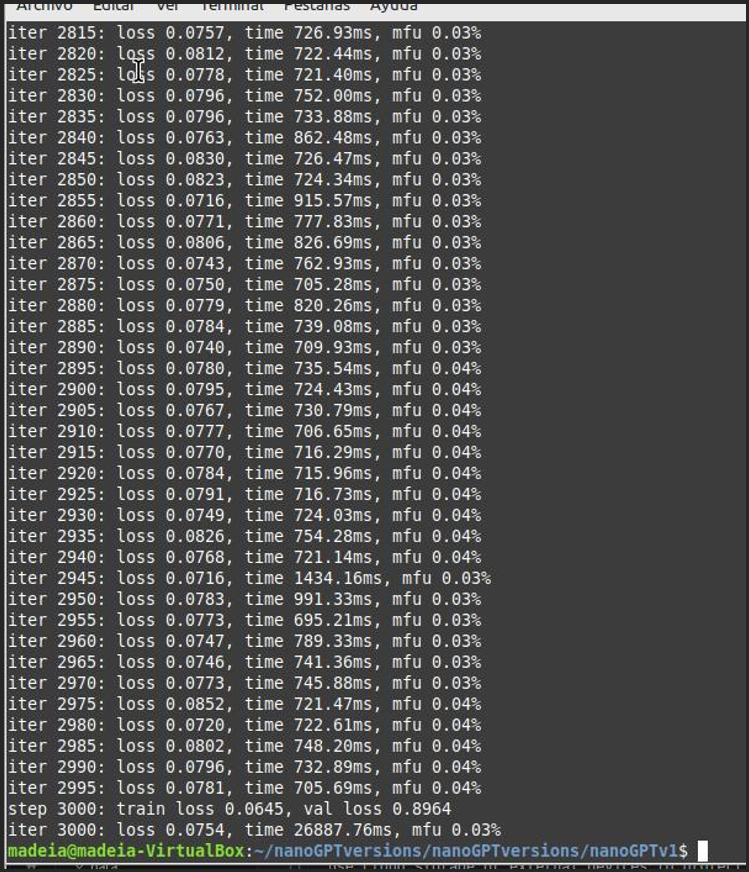
\includegraphics[width=0.6\linewidth]{./rp/06-cp.png} 
	\caption{Proceso de entrenamiento de modelo 2\cite{}}
	\label{figure:Resultado 1}  % assign a unique label to each figure 
\end{figure}
%----------------------------------------------------------------------------
\clearpage

\subsection{Validación del modelos}\label{section:Validación de prompt}
Durante la prueba 1 ejecuta el archivo \textbf{sample.py} que permite configurar las variaciones en las respuestas, los parámetros en este código permiten configurar la cantidad de tokens, su probabilidad siendo cero la más baja, la temperatura para que el modelo muestre aleatoriedad en la decodificación del texto. 
En esta seccion se realizan pruebas con las mismas consultas a los dos modelos en las categorías \textbf{Tips para protegerse sel phising}, {consejos para navegación segura}
\subsection{Validación del modelo 1}\label{section:Validación Modelo 2}
\subsubsection{ Prueba 1}\label{section:Prueba 1 config 2}
Durante la prueba 1 ejecuta el archivo \textbf{sample.py} que permite configurar las variaciones en las respuestas, los parametros en este código permiten configurar la cantidad de tokens, su probabilidad siendo cero la más baja, la temperatura para que el modelo muestre aleatoriedad en la decodificación del texto. Las configuraciones de la prueba uno establecen estos parámetros para obtener los tokens mas probables, matener una aleatoriedad en la respuesta y una máxima cantidad de tokens en quinientos.  
La consulta realizada es sobre 
Ejecución de pruebas
\subsubsection{ Prueba 1}\label{section:Modelo 1 Prueba1}
\begin{figure}[H]
	\centering % figure is centered on the page
	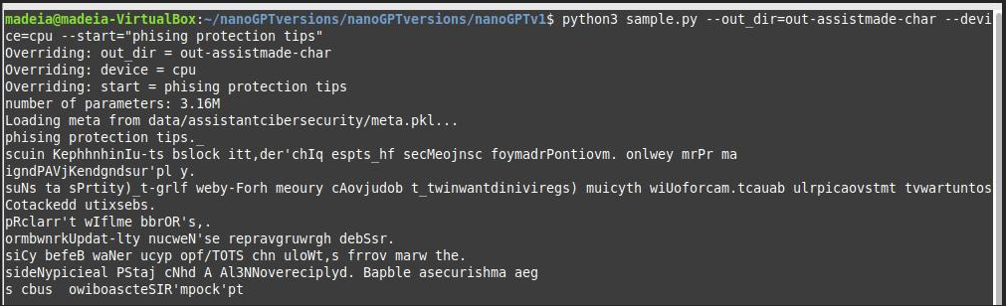
\includegraphics[width=0.60\linewidth]{./rp/07-cp.png} 
	\caption{Resultado de modelo 1 con temperatura 10 y probabilidad de tokens en 1, consulta sobre\cite{}}
	\label{figure:Result prueba 1 mol 1}  % assign a unique label to each figure 
\end{figure}
\subsubsection{ Prueba 2}\label{section:Modelo 1 Prueba2}
\begin{figure}[H]
	\centering % figure is centered on the page
	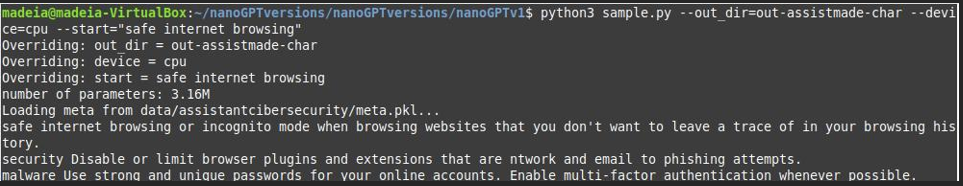
\includegraphics[width=0.60\linewidth]{./rp/08-cp.png} 
	\caption{Prueba 2 consulta sobre navegación segura en internet}
	\label{figure:Result modelo 1 prueba 2}  % assign a unique label to each figure 
\end{figure}
\subsubsection{ Prueba 3}\label{section:Prueba 3 mol 2}
\begin{itemize}
	\item   Top-k = 100
	\item   Temperatura = 1.2
	\item   Ma-new-tokens = 500
	\item   Prompt = python3 sample.py --out-dir=out-assistmade-char --device=cpu --start=" phising protection tips"
	\begin{figure}[H]
		\centering % figure is centered on the page
		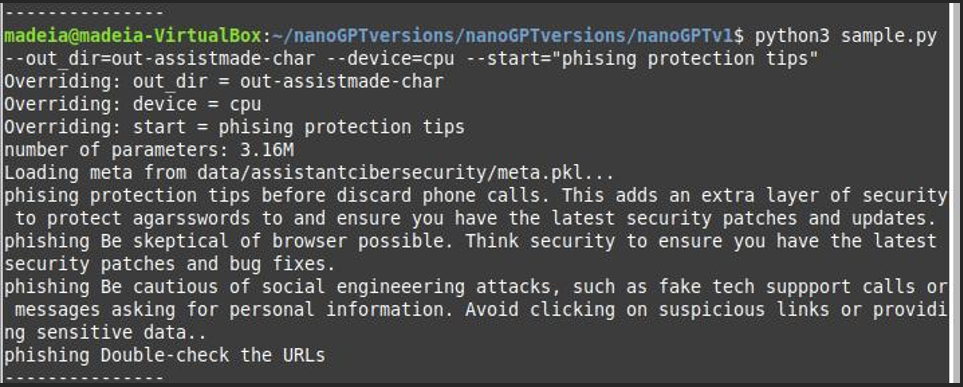
\includegraphics[width=0.60\linewidth]{./rp/09-cp.png} 
		\caption{Prueba 3 con configuración d probabilidad del token en 100 y temperatura 1.2}
		\label{figure:Result Prueba 3 mod 2}  % assign a unique label to each figure 
	\end{figure}
	\item   Prompt = python3 sample.py --out-dir=out-assistmade-char --device=cpu --start="safe internet browsing"
	\item   Prompt = python3 sample.py --out-dir=out-assistmade-char --device=cpu --start="computer security tips"
	\begin{figure}[H]
		\centering % figure is centered on the page
		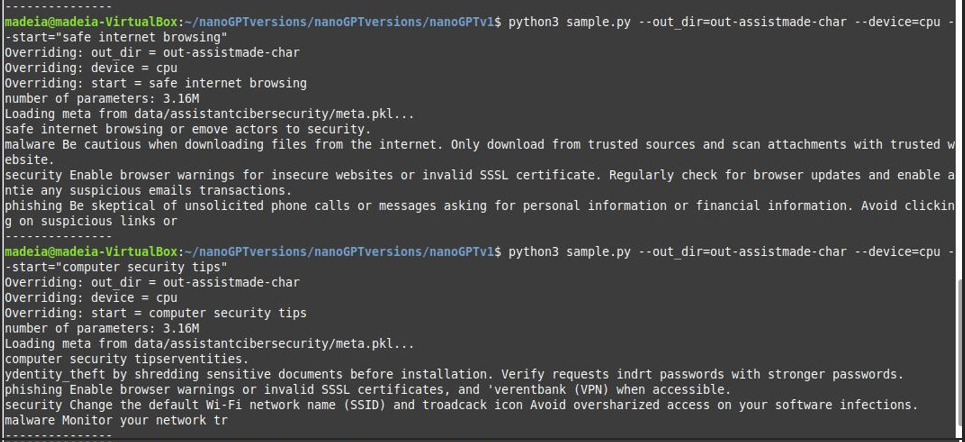
\includegraphics[width=0.65\linewidth]{./rp/10-cp.png} 
		\caption{Resultados de la Prueba 3.2 y 3.3\cite{}}
		\label{figure:Resultado 3.2}  % assign a unique label to each figure 
	\end{figure}
	\item   Prompt = python3 sample.py --out-dir=out-assistmade-char --device=cpu --start="computer security tips"
	\begin{figure}[H]
		\centering % figure is centered on the page
		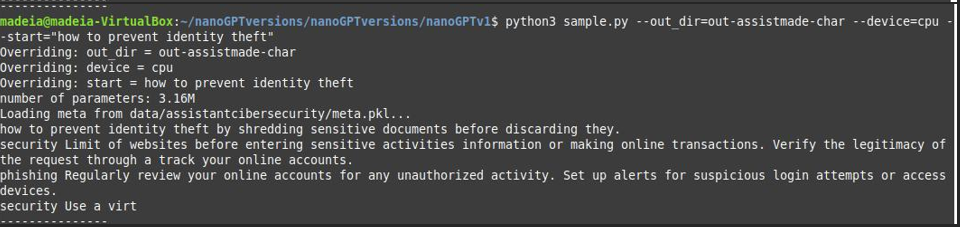
\includegraphics[width=0.65\linewidth]{./rp/11-cp.png} 
		\caption{Resultados de la Prueba 3.4\cite{}}
		\label{figure:Resultado 3.4}  % assign a unique label to each figure 
	\end{figure}
\end{itemize}
\subsubsection{ Prueba 4}\label{section:Adaptación de modelo nanoGPT}
\begin{itemize}
	\item   Top-k = 100
	\item   Temperatura = 1.1
	\item   Ma-new-tokens = 500
	\item   Prompt = python3 sample.py --out-dir=out-assistmade-char --device=cpu --start=" phising protection tips"
	\begin{figure}[H]
		\centering % figure is centered on the page
		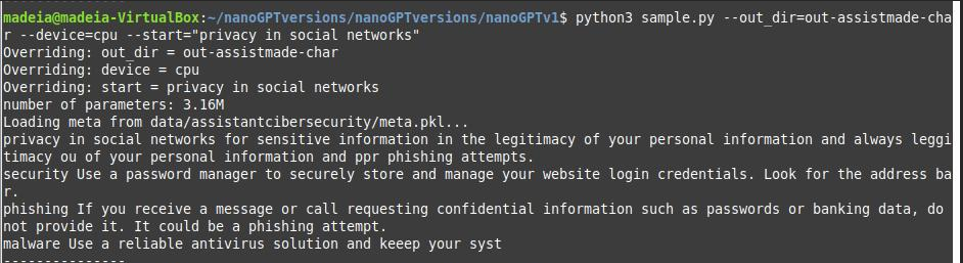
\includegraphics[width=0.65\linewidth]{./rp/12-cp.png} 
		\caption{Resultados de la Prueba 4.1\cite{}}
		\label{figure:Resultado 4 1}  % assign a unique label to each figure 
	\end{figure}
	\item   Prompt = python3 sample.py --out-dir=out-assistmade-char --device=cpu --start="computer security tips"
	\begin{figure}[H]
		\centering % figure is centered on the page
		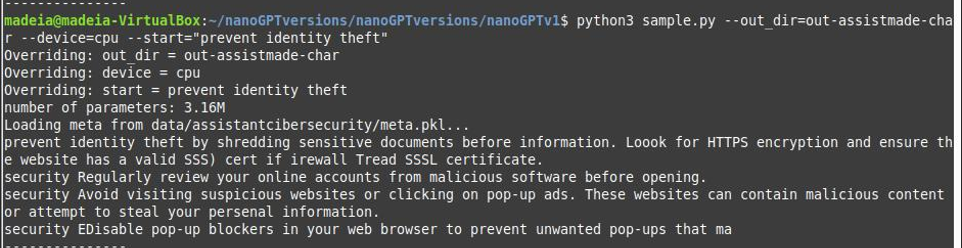
\includegraphics[width=0.65\linewidth]{./rp/13-cp.png} 
		\caption{Resultados de la Prueba 4.2\cite{}}
		\label{figure:Resultado prueba 4 2}  % assign a unique label to each figure 
	\end{figure}
	\item   Prompt = python3 sample.py --out-dir=out-assistmade-char --device=cpu --start="computer security tips"
	\begin{figure}[H]
		\centering % figure is centered on the page
		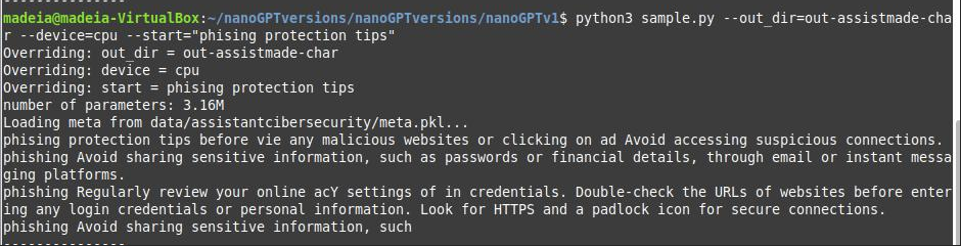
\includegraphics[width=0.65\linewidth]{./rp/14-cp.png} 
		\caption{Resultados de la Prueba 4.3\cite{}}
		\label{figure:Result prueba 4}  % assign a unique label to each figure 
	\end{figure}
\end{itemize}
%---------------------------------------------------------------------------
\subsubsection{ Pruebas de modelo 2}\label{section:Validación del prototipo}
Durante la prueba 1 se mantienen ejecuta el archivo \textbf{sample.py} que permite configurar las variaciones en las respuestas, los parametros en este código permiten configurar la cantidad de tokens, su probabilidad siendo cero la más baja, la temperatura para que el modelo muestre aleatoriedad en la decodificación del texto. Las configuraciones de la prueba uno establecen estos parámetros para obtener los tokens mas probables, matener una aleatoriedad de 1.2 y una máxima cantidad de tokens en quinientos.  La consulta realizada es sobre \textbf{Tips para protegerse sel phising}, {consejos para navegación segura}
Ejecución de pruebas
\begin{figure}[H]
   \centering % figure is centered on the page
       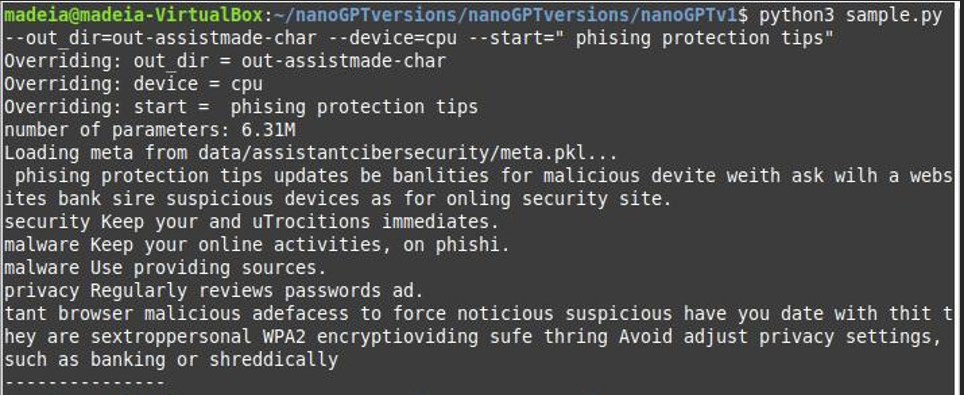
\includegraphics[width=0.65\linewidth]{./rp/16-cp.png} 
   \caption{Resultados de la Prueba 1\cite{}}
  \label{figure:Prueba1}  % assign a unique label to each figure 
\end{figure}
\begin{figure}[H]
   \centering % figure is centered on the page
       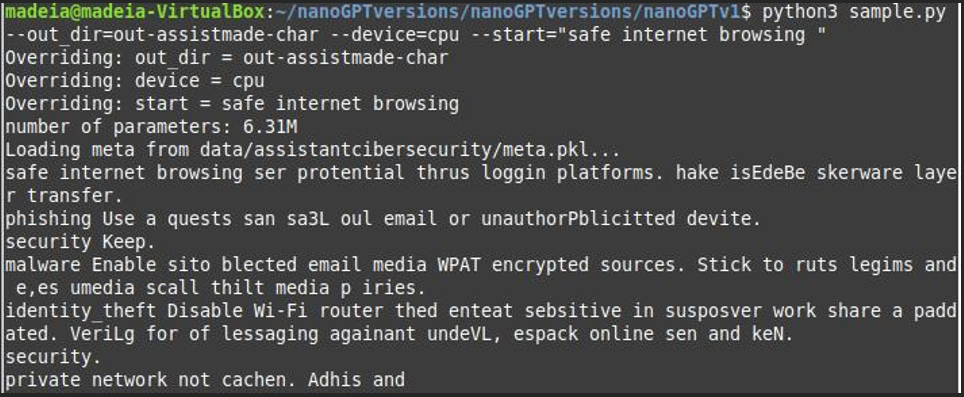
\includegraphics[width=0.65\linewidth]{./rp/17-cp.png} 
   \caption{Resultados de la Prueba 2\cite{}}
  \label{figure:Prueba2}  % assign a unique label to each figure 
\end{figure}
\begin{figure}[H]
   \centering % figure is centered on the page
       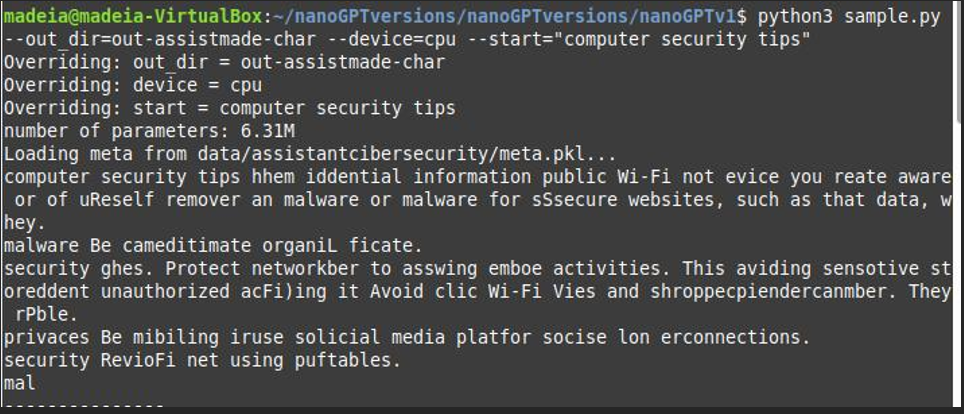
\includegraphics[width=0.65\linewidth]{./rp/18-cp.png} 
   \caption{Resultados de la Prueba 3\cite{}}
  \label{figure:Resultado prueba 3}  % assign a unique label to each figure 
\end{figure}
\begin{figure}[H]
   \centering % figure is centered on the page
       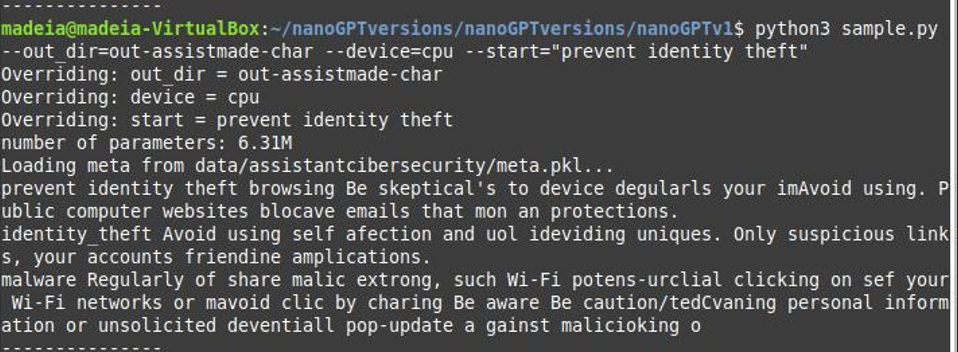
\includegraphics[width=0.65\linewidth]{./rp/19-cp.png} 
   \caption{Resultados de la Prueba 4\cite{}}
  \label{figure:Resultado prueba 4}  % assign a unique label to each figure 
\end{figure}
%-----------------------------------------------------------------------------   

%------------------------------------------------------------------------------

